
Another possible way of refining the \pipulse is the \textit{Flipping} experiment.\\
In particular, if the Ramsey experiment is used to fine tune the frequency, the Flipping experiment can be used to fine tune the amplitude, sometimes with notable differences in respect to the value found with Rabi.

In this context, we define a flip as two consecutive \pipulses that, in the ideal condition, should in the end lead to the initial state.\\
For the experiment, we choose a maximum number of flips $M$ and step number $S$.
We now have all the elements to perform the experiment:
\begin{itemize}
    \item with the qubit in $\ket 0$, we apply a \pihpulse;
    \item we apply $N$ flips (with $N\in [0,M]$ with steps of S);
    \item we measure;
    \item we repeat the experiment with a higher number of flips.
\end{itemize}

In the ideal case we should see just a straight line, always being in a superposition state (so in the middle point between the two amplitude states).
In the case of a wrong amplitude, we encounter oscillations.
We can perform a fit analog to the Ramsey experiment, or even proceed by manual tries, since the experiment is generally extremely fast (after all, there is no scan). 

In \cref{fig:flipping} we can see a possible plot for the flipping experiment.
\begin{figure}[ht]
    \centering
    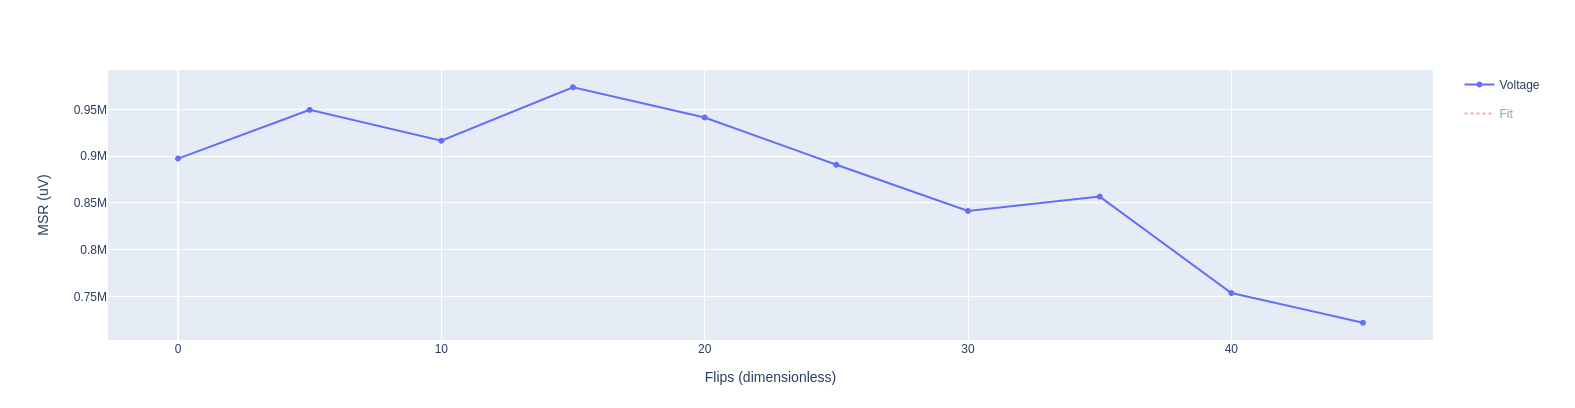
\includegraphics[width=\textwidth]{characterization/figures/flipping.png}
    \caption{Plot of a flipping experiment.}
    \label{fig:flipping}
\end{figure}
In this case the amplitude is almost correct, since we cannot see any clear oscillation, but can for sure be fine tuned to remove the present "decay".

While this experiment can be interesting, it has the problem of involving a large number of gates and this may  cause memory problems in the control system.

\experimentrecap
{Flipping}
{drive calibration}
{fine tuned qubit/drive frequency,\\characteristic dephasing time $T_2$ ($T_2^\star$)}
{after a \pihpulse, an increasing number of flips is executed (a couple of \pipulse). If the drive frequency is correct, the resulting plot will just present exponential decay, otherwise an oscillation from which we can extract the correct frequency.}






